\section*{\centering Содержание работы}
\addcontentsline{toc}{chapter}{Содержание работы}

Во \textbf{введении} определены актуальность избранной темы, степень ее разработанности, цели и задачи диссертационной работы, ее научная новизна, теоретическая и практическая значимость, методология диссертационного исследования, положения, выносимые на защиту, степень достоверности полученных результатов, апробация результатов и личный вклад автора. 

В {\bf главе 1} описан метод исследования. В работе движение жидкости моделируется численными решениями полных трехмерных уравнений Навье-Стокса. 
%Существенным достоинством численных методов при изучении механизмов турбулентности является то, что расчет дает полную информацию о течении. Подробный численный анализ ряда пристенных течений показал, что численные решения уравнений Навье-Стокс с высокой точностью воспроизводят наблюдаемые в экспериментах особенности движения. Прямое численное моделирование зарекомендовало себя эффективным методом изучения пристенных турбулентных течений. 
Во введении к главе приведен краткий историко-литературный обзор развития численных методов для решения задач гидродинамики и краткий обзор подходов к прямому численному моделированию пристенных турбулентных течений. 

В \textbf{разделе 1.1} приведена постановка задачи. В работе рассматривается течение вязкой несжимаемой жидкости в прямой трубе круглого сечения. Течение описывается уравнениями Навье-Стокса и неразрывности.
%$$
%\pd{\v}{t} = - (\v \cdot \nabla) \v - \frac{1}{\rho}\grad p + \nu \nabla^2 \v,
%$$
%$$
%\nabla \cdot \v = 0,
%$$
%где $\v$ --- поле скорости, $p$ --- давление, $\rho$ и $\nu$ --- постоянные плотность жидкости и кинематический коэффициент вязкости, $t$ --- время. 
На стенках трубы, имеющей радиус $R$, ставится условие прилипания. В продольном направлении на поле скорости накладывается условие периодичности с периодом $L_x$. Жидкость приводится в движение внешним градиентом давления, который определяется из условия постоянства средней скорости $U_m$. 

Задача решается в безразмерных переменных. В качестве основных единиц измерения выступают радиус трубы $R$, максимальная скорость течения Пуазейля $U = 2U_m$ и плотность жидкость $\rho$. Безразмерным параметром системы является число Рейнольдса $ \Re = {R U}/{\nu}$, где $\nu$ --- кинематический коэффициент вязкости.

Постановка задачи традиционна для прямого расчета развитых турбулентных течений в трубах и каналах. В такой постановке удается воспроизводить характеристики течения, устанавливающегося на большом удалении от входа в трубу, решая уравнения движения в ограниченной расчетной области. Условие периодичности вдоль трубы освобождает от необходимости устанавливать условия на входе и выходе из трубы. В тоже время, увеличивая длину периода $L_x$, можно минимизировать влияние этого условия на поток.

В \textbf{разделе 1.2} описан конечно-разностный метод решения поставленной задачи. Уравнения решаются в цилиндрической системе координат $(x,r,\theta)$. Дискретизация уравнений выполнена на перемежающихся сетках, что позволяет удобно аппроксимировать уравнения и граничные условия с сохранением аналогов ряда важных консервативных свойств исходной системы. Ребра сеток совпадают с координатными линиями. Дискретизация по пространственным переменным выполнена со вторым порядком точности. Для интегрирования по времени применен полунеявный метод Рунге-Кутты третьего порядка точности. Наиболее полно метод описан в (Nikitin, J. Comp. Phys. 2006).

\textbf{Раздел 1.3} посвящен практическим вопросам реализации вычислений. Пакет программ, реализующих численный метод, написан на языке программирования Fortran77. Помимо последовательного варианта программы реализован параллельный, позволяющий выполнять расчеты на кластерных вычислительных системах с распределенной памятью. Работа выполнена с использованием оборудования Центра коллективного пользования сверхвысокопроизводительными вычислительными ресурсами МГУ имени М.В.\,Ломоносова. 
%Значительная часть кода, необходимого при анализе полученных результатов и управлении численными экспериментами, в том числе реализующая метод продолжения по параметру, была написана на высокоуровневом языке Python. 

В \textbf{разделе 1.4} приведены результаты расчетов движения жидкости в круглой трубе в диапазоне $1670 \leqslant \Re \leqslant 2800$ в достаточно протяженной расчетной области для того, чтобы воспроизвести явление пространственной локализации турбулентности. Турбулентность в расчетах принимает форму локализованных структур, характеристики которых совпадают с характеристиками турбулентных порывов, приведенными в литературе. Это подтверждает адекватность численного метода целям работы и качество его программной реализации. 

\textbf{Глава 2} посвящена исследованию модельного порыва --- предельного решения на сепаратрисе, отделяющей в фазовом пространстве области притяжения решений, соответствующих ламинарному и турбулентному режимам течения. Во введении приведен краткий обзор работ, посвященных анализу решений на сепаратрисе в круглой трубе. Основные результаты, приведенные в главы, опубликованы в работах автора диссертации \cite{MZG2015, Kazan2015, KMU2015}.

В \textbf{разделе 2.1} описан метод получения модельного порыва. Предварительно найденное турбулентное решение $\v_{turb}(\x,t)$ используется в итерационной процедуре отыскания предельного решения на сепаратрисе. Задача решается с начальным условием
\begin{equation} \label{edge_init_eq}
\v(\x,t=0) = \v_{Pois}(\x)+\alpha(\v_{turb}(\x,t=t_0) - \v_{Pois}(\x)),
\end{equation}
где $\v_{Pois}=(1-r^2,0,0)$ --- течение Пуазейля, $t_0$ --- некоторый фиксированный момент времени, $\alpha$ --- скалярный параметр. Значение $\alpha=0$ соответствует нулевому возмущению, и решением при $t > 0$ остается течение Пуазейля. Выбирая $\alpha=1$, уже в начальный момент времени реализуется турбулентный режим, который сохраняется при $t > 0$. При промежуточных значениях $\alpha$ происходит стремление решения либо к одному, либо к другому режиму. Применяя метод деления пополам, мы постепенно отыскиваем то значение $\alpha$, при котором решение эволюционирует на сепаратрисе, разделяющей области притяжения двух режимов течения. На рисунке \ref{bisection_pic} представлены графики $A(t)$ – среднеквадратичного по всему объему отклонения поля скорости от течения Пуазейля для нескольких значений $\alpha$, демонстрирующие сходимость итерационного процесса. При уточнении значения $\alpha$ продлевается длительность балансирования решения на сепаратрисе.

\begin{figure}
\center{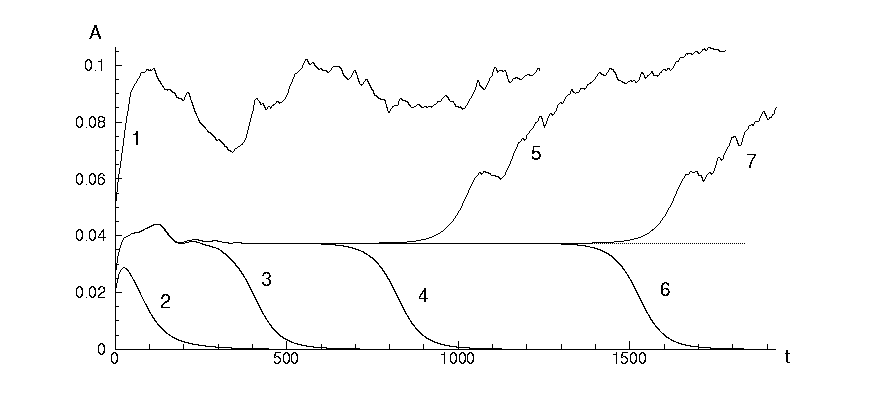
\includegraphics[width=1\linewidth]{bisection.png}}
\caption{Итерационный процесс построения решения на сепаратрисе.}
\label{bisection_pic}
\end{figure}

В согласии с (Avila et al., 2013), при $\Re=2200$ и дополнительных условиях диаметральной симметричности и $\pi$-периодичности в угловом направлении решение на сепаратрисе постепенно выходит на условно периодический режим. Предельное решение на сепаратрисе описывает пространственно локализованную структуру длиной около $40R$, перемещающуюся вдоль трубы со скоростью $c=0.69U$. В подвижной системе отсчета поле скорости в каждой точке испытывает периодические колебания с периодом $T=60R/U$. 

Визуализация мгновенного поля скорости модельного порыва приведена на рисунке \ref{3D_img}(б). Представлены области пониженной и повышенной на $0.1U$ скорости относительно течения Пуазейля. На рисунке \ref{3D_img}(а), для сравнения, приведена аналогичная визуализация для турбулентного порыва. Поток направлен слева направо. И в турбулентном, и модельном порывах наблюдаются вытянутые вдоль потока области, скорость внутри которых существенно выше или ниже среднего значения --- так называемые полосы повышенной и пониженной скорости. В отличии от турбулентного порыва в модельном порыве полосы сохраняют свое положение в пространстве и испытывают лишь незначительные колебания около положения равновесия. 

\begin{figure}[h]
\center{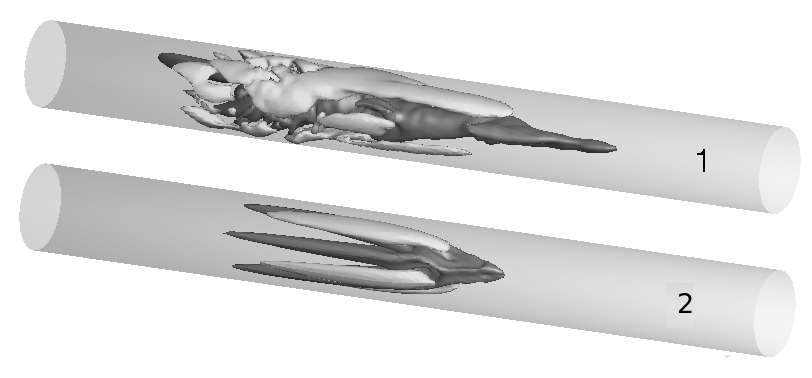
\includegraphics[width=1\linewidth]{autoref_3D_cmp.png}}
\caption{Визуализация численных расчетов турбулентных порывов.}
\label{3D_img}
\end{figure}


Сравнение характеристик модельного порыва, полученных на нескольких расчетных сетках и в работах других авторов, позволяет сделать вывод, что найденное численно решение аппроксимирует соответствующее ему решение уравнений Навье-Стокса и не зависит от выбора численного метода и параметров расчета. Решение действительно является локализованным в пространстве, так как изменение протяженности расчетной области не влияет на протяженность локализованной структуры и временной период. 


В \textbf{разделе 2.2} описаны основные свойства модельного порыва. В подвижной системе отсчета поле скорости модельного порыва $\v$ представляется в виде суперпозиции стационарной составляющей $\V = \overline{\v}^t$ и колебательной $\v_n = \v - \V$. Черта над выражением обозначает осреднение по указанной переменной. Стационарная составляющая, в свою очередь, представляется в виде суперпозиции осесимметричной $\V_{2D}(\x) = \overline{\V}^{\theta}$ и трехмерной $\V_{3D}(\x) = \V - \V_{2D}$. 

\begin{figure}[h]
\center{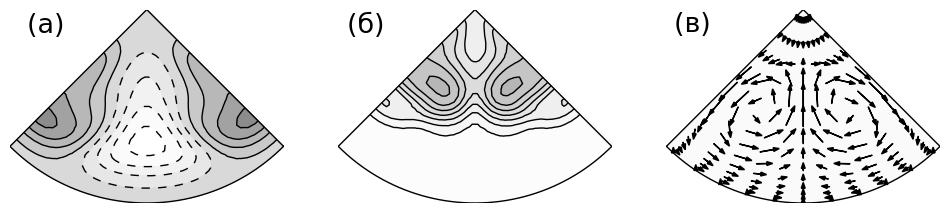
\includegraphics[width=1\linewidth]{mp_cs.png}}
\caption{Поле скорости модельного порыва}
\label{mp_cs_pic}
\end{figure}

В трехмерную стационарную составляющую движения $\V_{3D}$ попадают полосы повышенной и пониженной скорости. Изолинии $V_{x, 3D}$ в поперечном сечении трубы, где колебаний имеют существенную амплитуду, изображено на рисунке~\ref{mp_cs_pic}(a). В силу наложенных условий симметрии расчет проводится в одной четверти трубы. В каждом сечении трубы полосы пониженной скорости ($V_{x,3D} < 0$, прерывистые линии) проходят через центр расчетной области. Полосы повышенной скорости ($V_{x,3D} > 0$, сплошные линии) попадают на границы расчетной области в угловом направлении. 

На рисунке \ref{mp_cs_pic}(б) приведено распределение среднеквадратичной амплитуды пульсационной составляющей движения $\v_n$ в том же сечении трубы. Пульсации имеют существенную амплитуду между полосами повышенной и пониженной скорости, а также между полосой ускорения и осью трубы. Пульсационная составляющая движения $\v_n$ по форме напоминает бегущую волну. Её фазовая скорость близка к $0.77U$, а длину можно оценить в $5R$. 

В \textbf{разделе 2.3} показано, что за образование полос повышенной и пониженной скорости ответственен лифтап (lift-up) эффект, связанный с движением жидкости в перпендикулярной к основному потоку плоскости. Частицы жидкости, перемещающиеся от стенки в сторону оси трубы, приносят дефект скорости и образуют полосу замедления, а частицы, двигающиеся в противоположном направлении --- от оси к стенке, образуют полосу ускорения.
Векторное поле поперечной компоненты среднего течения $\V_{3D}$ приведено на рисунке \ref{mp_cs_pic}(в). Оно соответствует существованию в потоке стационарных продольных вихрей, поддерживающих существование полос. 

В \textbf{разделе 2.4} показано, что пульсации возникают в результате линейной неустойчивости среднего течения. Для того, чтобы установить это, линеаризованные относительно возмущений уравнения с некоторыми случайными начальными условиями интегрировались по времени до выхода решения на режим экспоненциального изменения. Обнаружено, что $\V$ неустойчиво. Растущее возмущение $\v'_1 \sim e^{(\lambda+i\omega)t}$ имеет инкремент нарастания $\lambda=0.012$ и частоту $\omega=0.116$, близкую к частоте колебаний $2\pi/60=0.105$ в модельном порыве. Поле скорости растущего решения $\v'_1$ качественно повторяет основные особенности поля скорости пульсационной составляющей движения модельного порыва $\v_n$. 

Отметим, что поле скорости $\V$ является существенно трехмерным и все три компоненты скорости отличны от нуля. Численные методы позволяют исследовать устойчивость такого поля скорости. Хотя значения $V_r$ и $V_\theta$ на порядок ниже значения $V_x$, их учет необходим для адекватного описания механизма поддержания продольных вихрей, описанного в главе 3.

В \textbf{разделе 2.5} рассматривается вопрос влияния продольной неоднородности среднего течения на форму пульсаций. Для этого на устойчивость исследуются однородные вдоль трубы поля скорости $\U_i = \V\big|_{x=x_i}$, повторяющее среднее течение в сечениях $x = x_i$ из области, в которой пульсации имеют существенную амплитуду. Показано, что продольная неоднородность стационарной составляющей движения не является необходимым условием для возникновения пульсаций и не влияет существенным образом на характеристики пульсационной составляющей движения. 

В \textbf{разделе 2.6} на основе уравнений движения анализируется вклад каждой из компонент движения в производство кинетической энергии других компонент движения, что позволяет более строго обосновать сделанные в главе выводы о взаимодействии между различными компонентами движения. Также полученные результаты подтверждают, что выделены и учтены все существенные взаимодействия между компонентами движения. 

В \textbf{разделе 2.7} приведены выводы по главе. 

\textbf{Глава 3} посвящена обнаруженному в работе механизму поддержания продольных вихрей. В \textbf{разделах 3.1 -- 3.3} механизм дается на примере решения, имеющего вид бегущей волны. Это решение периодично вдоль потока и стационарно в сопутствующей системе отсчета. Простота его поведения позволяет в более строгой форме показать ряд особенностей движения, обеспечивающих работу механизма. 

В \textbf{разделе 3.4} проводится обобщение механизма поддержания продольных вихрей на модельный порыв. 
Прояснить процесс поддержания продольных вихрей позволяет анализ уравнения эволюции средней продольной завихренности
\begin{multline}\label{OX_eq}
\pd{\Omega_x}{t} + (V_x - c_f)\pd{\Omega_x}{x} + V_r \pd{\Omega_x}{r} + \frac{V_\theta}{r} \pd{\Omega_x}{\theta} - \nu\nabla^2\Omega_x= \Omega_x \pd{V_x}{x} + \Omega_r \pd{V_x}{r} + \\ + \frac{\Omega_\theta}{r} \pd{V_x}{\theta}
 - \overline{v'_x \pd{\omega'_x}{x}}^t - \overline{v'_r \pd{\omega'_x}{r}}^t - \overline{\frac{v'_\theta}{r} \pd{\omega'_x}{\theta}}^t
 + \overline{\omega'_x \pd{v'_x}{x}}^t + \overline{\omega'_r \pd{v'_x}{r}}^t + \overline{\frac{\omega'_\theta}{r} \pd{v'_x}{\theta}}^t,
\end{multline}
в котором $\Om = (\Omega_x, \Omega_r, \Omega_\theta)$ и $\om' = (\omega'_x, \omega'_r, \omega'_\theta)$ --- средняя и пульсационная составляющие вектора завихренности $\om = \rot \v$, $c_f$ --- скорость перемещения системы отсчета. Система находится в равновесии и средняя завихренность во времени не меняется. Источниковые слагаемые в правой части уравнения компенсируются конвективными и вязкими слагаемыми в левой. Анализ уравнения \eqref{OX_eq} показал, что два слагаемых в правой части, а именно
\begin{equation}\label{OXgen_terms}
- \overline{v'_x \frac{\d \omega'_x}{\d x}}^t + \overline{ \omega'_x \frac{\d v'_x}{\d x} }^t,
\end{equation}
вносят определяющий вклад в производство средней продольной завихренности. 

Для представления количественных данных обратимся к уравнения эволюции квадрата $\Omega_x$, полученному умножением \eqref{OX_eq} на $2\Omega_x$. Положительный или отрицательный знак у выражений в правой части этого уравнения показывает соответственно положительный или отрицательный вклад этого члена в изменение $\Omega^2_x$, а следовательно, и в интенсивность поперечного движения. Распределение $\Omega^2_x$ по сечению трубы представлено на Рисунке \ref{OXgen_pic}(a). Область концентрации $\Omega_x$ расположена между полосами повышенной и пониженной скорости и соответствюут расположению продольных вихрей на Рисунке \ref{mp_cs_pic}(в). Соответствующее сумме \eqref{OXgen_terms} распределение в уравнении для $\Omega^2_x$ представлено на Рисунке \ref{OXgen_pic}(б), а вклад остальных слагаемых правой части \eqref{OX_eq} показан на Рисунке \ref{OXgen_pic}(в). Распределение генерации $\Omega^2_x$ выделенными в \eqref{OXgen_terms} членами практически совпадает по форме с распределением $\Omega^2_x$, тогда как вклад остальных членов не имеет выраженного распределения и более чем на порядок уступает по суммарному вкладу в генерацию $\Omega^2_x$. Таким образом, нет сомнения в том, что стационарные продольные вихри возникают за счет действия слагаемых \eqref{OXgen_terms}.

\begin{figure}
\center{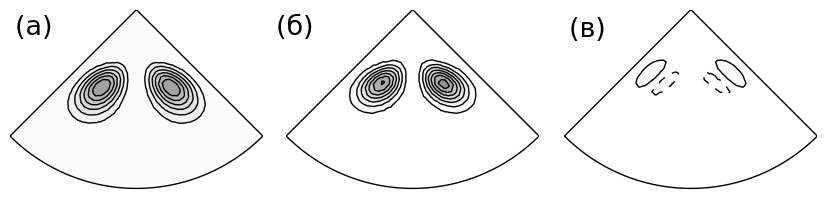
\includegraphics[width=1\linewidth]{autoref_OXgen.png}}
\caption{Механизм генерации продольных вихрей}
\label{OXgen_pic}
\end{figure}

Между собой слагаемые \eqref{OXgen_terms} практически равны. Это значит, в частности, что колебания $\partial v'_x / \partial x$ и $\omega'_x$ положительно коррелированы в области концентрации положительной $\Omega_x$ и отрицательно коррелированы в области концентрации отрицательной $\Omega_x$. То же относится и к колебаниям $-v'_x$ и $\partial \omega'_x / \partial x$. Выявить механизм формирования такой связи позволяет анализ уравнения эволюции $\omega'_x$:
\begin{multline}\label{ox1_eq}
\pd{\omega'_x}{t} + (V_x - c_f)\pd{\omega'_x}{x} + V_r \pd{\omega_x'}{r} + \frac{V_\theta}{r} \pd{\omega'_x}{\theta} 
- \nu\nabla^2\omega'_x = - v'_x \pd{\Omega_x}{x} - v'_r \pd{\Omega_x}{r} - \\ - \frac{v'_\theta}{r} \pd{\Omega_x}{\theta} 
+ \Omega_x \pd{v'_x}{x} + \Omega_r \pd{v'_x}{r} + \frac{\Omega_\theta}{r} \pd{v'_x}{\theta}
+ \omega'_x \pd{V_x}{x} + \omega'_r \pd{V_x}{r} + \frac{\omega'_\theta}{r} \pd{V_x}{\theta} - \\ 
- v'_x \pd{\omega'_x}{x} - v'_r \pd{\omega'_x}{r} - \frac{v'_\theta}{r} \pd{\omega'_x}{\theta} 
+ \omega'_x \pd{v'_x}{x} + \omega'_r \pd{v'_x}{r} + \frac{\omega'_\theta}{r} \pd{v'_x}{\theta} + \\
+ \overline{v'_x \pd{\omega'_x}{x}}^t + \overline{v'_r \pd{\omega'_x}{r}}^t + \overline{\frac{v'_\theta}{r} \pd{\omega'_x}{\theta}}^t
- \overline{\omega'_x \pd{v'_x}{x}}^t - \overline{\omega'_r \pd{v'_x}{r}}^t - \overline{\frac{\omega'_\theta}{r} \pd{v'_x}{\theta}}^t.
\end{multline}
%Умножение \eqref{ox1_eq} на $2\omega'_x$ и последующее осреднение по времени дает уравнение баланса среднего квадрата пульсаций продольной завихренности $\overline{\omega'_x\omega'_x}^t$. Слагаемые в этом уравнении не зависят от времени. Как и в предыдущем случае, с
Среди всех источниковых слагаемых в правой части \eqref{ox1_eq} также удалось выделить существенные, ответственные за возникновение пульсаций $\omega'_x$. Как показано в работе, в области формирования продольных вихрей за образование $\omega'_x$ отвечает выделенное ниже слагаемое.
\begin{equation}\label{ox1gen_main_terms}
\frac{\d \omega'_x}{\d t} = \Omega_x \frac {\d v'_x}{\d x} + ...
\end{equation}
Выделенное в \eqref{ox1gen_main_terms} слагаемое отвечает за перераспределение уже существующей стационарной продольной завихренности $\Omega_x$ пульсационной составляющей продольной скорости $v'_x$ (эффект сжатия/растяжения вихревых трубок). Оно стремится произвести пульсации $\omega'_x$, пропорциональные $\d v'_x / \d x$, причем коэффициентом пропорциональности выступает средняя продольная завихренность. Соответственно, механизм включается в областях концентрации~$\Omega_x$. В области расположения положительного вихря производимые пульсации $\omega'_x$ положительно пропорциональны пульсациям $\d v'_x / \d x$, а в области расположения отрицательного вихря --- отрицательно пропорциональны. Таким образом обеспечивается максимально возможная эффективность производства средней продольной завихренности нужного знака посредством второго из слагаемых \eqref{OXgen_terms}. Пульсации $-v'_x$ и $\d \omega'_x / \d x$ отказываются также согласованы нужным образом, и первое слагаемое \eqref{OXgen_terms} оказывается равно второму.

Фазовая скорость бегущей волны, соответствующей пульсационной составляющей движения, совпадает со средней скоростью жидкости в области формирования продольных вихрей. По этой причине формируемые \eqref{ox1gen_main_terms} пульсации $\omega'_x$, перемещаясь вниз по потоку за счет конвекции, остаются в фазе с порождающими их пульсациями $\partial v'_x / \partial x$.

В \textbf{разделе 3.5} приведены выводы по главе. Основные результаты главы опубликованы в работах автора диссертации  \cite{MZG2017, Lomonosov2018, Ob2018}.

 

%В \textbf{главе 4} поднимается вопрос об универсальности полученных при исследовании модельного порыва результатов. Для ответа на него рассчитаны и исследованы отличные от модельного порыва решения уравнений Навье-Стокса. 
%В частности, исследованы условно-периодические решения уравнений Навье-Стокса с пространственно локализованной структурой, полученные продолжением решения, соответствующего модельному порыву, по параметру. Также исследовано три семейства решений, имеющих вид бегущей волны. Одно описывает течение в круглой трубе, два других --- в плоском канале. Все исследованные решения воспроизводят общий механизм поддержания колебаний, что подкрепляет представление о его универсальности.

В \textbf{разделе 4.1} описан метод Ньютона для нахождения условно-периодических решений уравнений Навье-Стокса и решений в виде бегущей волны, как частного случая условно-периодических. Приближение к решению возникающей на каждой итерации метода Ньютона линейной системы ищется в подпространствах Крылова методом минимизации невязки. 
%Поиск приближения к решению в подпространствах Крылова позволяет существенно снизить требования к вычислительным ресурсам, необходимым для применения метода Ньютона. 
На применении метода Ньютона основан метод продолжения по параметру. Когда одно решение известно, оно используется в качестве начального приближения к решению при близком значении параметров, с которыми метод сходится. Затем найденное решение используется в качестве начального приближения к новому решению, и т.д. Так строится цепочка решений, связывающая решения с существенно различными значениями параметров --- решение продолжается по параметру.


В \textbf{разделе 4.2} приведены результаты продолжения модельного порыва по $\Re$, позволившего получить новые условно периодические решения уравнений Навье-Стокса с пространственно локализованной структурой. Решения принадлежат однопараметрическому множеству. Значения амплитуды трехмерной составляющей движения $a$ и скорости перемещения вдоль трубы $c$ как функции $\Re$ приведены на Рисунке \ref{contin_pic}. Жирные точки на графиках соответствуют исходному решению. При $\Re \approx 1400$ обнаружена точка бифуркации, в которой рождается две ветви решений. При каждом $\Re$, превышающем критическое значение, существует два решения, каждое из которых принадлежит свой ветви. 
% При меньших $\Re$ таких решений не существует. При больших $\Re$ существует две ветви решений, то есть при каждом значении $\Re$ существует два решения, каждое из которых принадлежит свой ветви. 
Ветвь, которой принадлежит исходное решение, называют нижней. Вторую ветвь называют верхней. Для верхней ветви характерна большая интенсивность пульсаций и меньшая скорость перемещения вдоль трубы. По этим и другим параметрам решения с верхней ветви оказывается ближе к турбулентному порву, чем исходное решение. Результаты согласуются с (Avila et al. 2013). 


\begin{figure}
\center{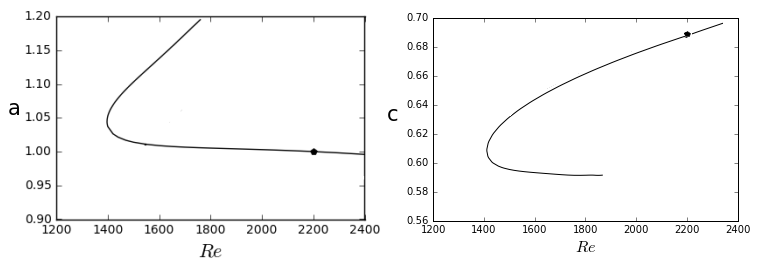
\includegraphics[width=0.9\linewidth]{autoref_contin.png}}
\caption{Продолжение модельного порыва по числу Рейнольдса}
\label{contin_pic}
\end{figure} 

В \textbf{разделе 4.3} выполнено исследование верхней ветви порожденного модельным порывом семейства условно-периодических решений. На Рисунке \ref{3D_ub_pic} приведена визуализация мгновенного поля скорости решения с верхней ветви. Несмотря на существенные количественные отличия, решения с верхней ветви воспроизводят тот же механизм поддержания колебаний, что и решение с нижней ветви. Поле скорости решения представляется в виде суперпозиции средней и пульсационной составляющих. Области повышенной и пониженной средней скорости представляют собой вытянутые вдоль потока полосы. На Рисунке \ref{ub_cs_pic}(a) приведены изолинии средней продольной скорости в поперечном сечении трубы, в котором пульсации имеют существенную амплитуду. В центральной части расчетной области, где изолинии находятся на большем удалении от стенки, проходит полоса пониженной скорости. При больших и меньших значениях $\theta$ находятся полосы повышенной скорости. Пульсации возникают в результате линейной неустойчивости среднего течения между соседними полосами повышенной и пониженной скорости. Угловую неоднородность среднего течения поддерживают продольные вихри, которым соответствуют области повышенных и пониженных значений средней продольной завихренности $\Omega_x$. Распределение $\Omega^2_x$ в том же сечении трубы приведено на Рисунке \ref{ub_cs_pic}(б). Определяющий вклад в производство $\Omega_x$ в уравнении \eqref{OX_eq} дают слагаемые \eqref{OXgen_terms}. Вклад слагаемых, соответствующих \eqref{OXgen_terms}, в производство $\Omega^2_x$ приведен на Рисунке \ref{ub_cs_pic}(в). Механизм образования пульсаций продольной завихренности в области формирования продольных вихрей также аналогичен выделенному в модельном порыве. 


\begin{figure}
\center{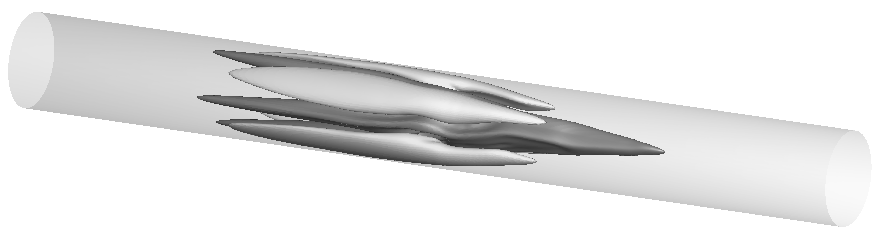
\includegraphics[width=0.9\linewidth]{ub_3D.png}}
\caption{Условно-периодическое решение с верхней ветви}
\label{3D_ub_pic}
\end{figure} 


\textbf{Разделы 4.4} и \textbf{4.5} посвящены анализу трехмерных бегущих волн в течении Гагена-Пуазейля и в плоском течении Пуазейля. Постановка задачи для плоского течения Пуазейля аналогична постановке для течения Гагена-Пуазейля. В каждом течении вид бегущей волны имеют предельные решения на сепаратрисе, найденные в непротяженной расчетной области. Также в плоском течении Пуазейля найдена устойчивая бегущая волна (при наложенных условиях симметрии). Методом продолжения по параметру рассчитаны соответствующие семейства решений. В отличии от модельного порыва, среднее поле скорости бегущей волны не зависит от продольной координаты --- полосы и продольные вихри имеют бесконечную протяженность. Решения достаточно существенно отличаются друг от друга, но, несмотря на это, механизм поддержания колебаний во всех трех семействах решений также аналогичен механизму поддержания колебаний в модельном порыве. 
%Отметим, что в некоторых решениях среднее поле скорости устойчиво к малым возмущениям, но и в этих случаях механизм передачи энергии в пульсационную составляющую движения, по-видимому, линейный, так как наиболее медленно затухающая собственная функция линейной задачи устойчивости повторяет форму и фазовую скорость пульсационной составляющей движения. Также в некоторых решениях слагаемое \eqref{ox1gen_main_terms} оказывается не единственным ответственным за производство $\omega'_x$ в области формирования продольных вихрей, но это слагаемое всегда имеет существенное значение и именно оно обеспечивает необходимую для поддержания продольных вихрей согласованность фаз между пульсациями $\omega'_x$ и $v'_x$. 
 
В \textbf{разделе 4.6} приведены выводы по главе. Основные результаты главы опубликованы в работах автора диссертации \cite{Vest18, KMU2016, Lomonosov2018, Lomonosov2017, LomRead2017, LomRead2016, Ob2018}. 



